\section{Test Results}
\subsection{Functionality}

\begin{center}
    \begin{tabular}{ | l | p{12cm} |}
    \hline
    Test 	 				& 		 Start the platform\\ \hline
	Produce  				& 		 This was tested by adding the platform as a startup service on a linux computer. When the computer was started the platform started.\\ \hline
	Expected Results  		& 		 The expected result is that the platform starts and connects to the network without any applications connected to it. \\ \hline
	Results 				& 		 As Expected\\ \hline
	Comments				& 		 This test shows that the requirement Platform as Daemon is met.\\ \hline
    \end{tabular}
\end{center}

\begin{center}
    \begin{tabular}{ | l | p{12cm} |}
    \hline
    Test 	 				& 		 Connect an application to the platform \\ \hline
	Produce  				& 		 This was done by starting a MediaSense application and connecting it to the background process from the previous test. The application registers itself with the platform and a connection to the platform is established. To see that the platform and the application is connected to each other the method getLocalhost() was called and the application printed this out in the output console. \\ \hline
	Expected Results  		& 		 The application connects to the platform and when the application register itself to the platform they are connected. When getLocalhost() is called the localhost for the platform should be printed in console. \\ \hline
	Results 				& 		 As Expected\\ \hline
	Comments				& 		 This shows that the old functionality still exists and work in the new artefact.\\ \hline
    \end{tabular}
\end{center}

\begin{center}
    \begin{tabular}{ | l | p{12cm} |}
    \hline
    Test 	 				& 		 Connect several applications to the platform\\ \hline
	Produce  				& 		 Ten applications were connected to the MediaSense daemon. All applications register themselves at the platform using the Interface method registerApplication.\\ \hline
	Expected Results  		& 		 All applications connects to the platform and connections are established without any errors.\\ \hline
	Results 				& 		 As Expected\\ \hline
	Comments				& 		 This test shows that several applications can connect to the platform. This test also shows that the requirement \emph{Several Applications} is met.\\ \hline
    \end{tabular}
\end{center}

\begin{center}
    \begin{tabular}{ | l | p{12cm} |}
    \hline
    Test 	 				& 		 Storing an UCI\\ \hline
	Produce  				& 		 One of the applications connected to the platform store an UCI by calling the method registerUCI.\\ \hline
	Expected Results  		& 		 A DuplicateUCICheckMessage is sent from the platform and a DuplicateUCICheckResponseMessage will be received when the UCI is stored in the network.\\ \hline
	Results 				& 		 As Expected\\ \hline
	Comments				& 		 This test shows that the functionality still works. The methods which are called are from the provided Interface. This shows that requirement \emph{Interface to applications} is met.\\ \hline
    \end{tabular}
\end{center}

\begin{center}
    \begin{tabular}{ | l | p{12cm} |}
    \hline
    Test 	 				& 		 Resolving an UCI\\ \hline
	Produce  				& 		 An application connected to the platform sends a ResolveMessage.\\ \hline
	Expected Results  		& 		 The application should call the method resolveUCI, causing the platform to send a ResolveMessage. When the message has been routed through the network a ResolveResponsMessage should be received by the platform and be passed to the application. \\ \hline
	Results 				& 		 As Expected\\ \hline
	Comments				& 		 The methods that are called are the methods from the provided Interface. This shows that requirement \emph{Interface to applications} is met.\\ \hline
    \end{tabular}
\end{center}

\begin{center}
    \begin{tabular}{ | l | p{12cm} |}
    \hline
    Test 	 				& 		 Sending a message\\ \hline
	Produce  				& 		 This was tested by building an application that sends NotifyMessages in response to a GetMessage. One of the connected applications sends a GetMessage and the application receiving this messages responds with a NotifyMessage.\\ \hline
	Expected Results  		& 		 A NotifyMessage should be received by the application that sent the GetMessage.\\ \hline
	Results 				& 		 As Expected\\ \hline
	Comments				& 		 The methods that are called are the methods from the provided Interface. This shows that the requirement \emph{Interface to applications} is met. \\ \hline
    \end{tabular}
\end{center}

\begin{center}
    \begin{tabular}{ | l | p{12cm} |}
    \hline
    Test 	 				& 		 Application crash with several application connected to platform\\ \hline
	Produce  				& 		 Connect several applications to a platform on one device. Make one of the applications crash by throwing an exception. A peer message was then sent to all applications connected to the platform.\\ \hline
	Expected Results  		& 		 Platform should still be working. No other applications connected to the platform should be affected by the crash. Messages should still be able to be sent and received by the platform.\\ \hline
	Results 				& 		 As Expected\\ \hline
	Comments				& 		 This shows that the requirement \emph{Application independent} is met.\\ \hline
    \end{tabular}
\end{center}

\begin{center}
    \begin{tabular}{ | l | p{12cm} |}
    \hline
    Test 	 				& 		 Send peer scope message\\ \hline
	Produce  				& 		 Sending a NotifyMessage from an application with the scope PEER. \\ \hline
	Expected Results  		& 		 All applications on the receiving node should get this NotifyMessage.\\ \hline
	Results 				& 		 As Expected\\ \hline
	Comments				& 		 Requirement \emph{Message with scope} is met.\\ \hline
    \end{tabular}
\end{center}

\begin{center}
    \begin{tabular}{ | l | p{12cm} |}
    \hline
    Test 	 				& 		 Send application scope message\\ \hline
	Produce  				& 		 Sending a NotifyMessage from an application with the scope APPLICATION and the application ID as an argument. \\ \hline
	Expected Results  		& 		 Application with the specific ID should get the notifyMessage. \\ \hline
	Results 				& 		 As Expected\\ \hline
	Comments				& 		 Requirement \emph{Message with scope} is met.\\ \hline
    \end{tabular}
\end{center}

\begin{center}
    \begin{tabular}{ | l | p{12cm} |}
    \hline
    Test 	 				& 		 Connect an application to an external MediaSense platform\\ \hline
	Produce  				& 		 The platform was started on one computer and an application running on another computer connects to the platform by getting its reference from the RMI registry.\\ \hline
	Expected Results  		& 		 Applications can communicate with the platform running on a PC. \\ \hline
	Results 				& 		 As Expected\\ \hline
	Comments				& 		 Requirement gateway is met. \\ \hline
    \end{tabular}
\end{center}

\subsection{Resource Usage Measurement}

\subsubsection{Memory Usage Old MediaSense Version}
\begin{center}
    \begin{tabular}{ | l | p{9cm} | l |}
    \hline
    No. Apps 								& Memory Usage 																									& Total\\ \hline
    0 													& 0 MB 																											& 0 MB\\ \hline
    1 													& 70.4 MB 																										& 70.4 MB\\ \hline
    2 													& 68.8 MB + 70.4 MB																								& 139.2 MB\\ \hline
    3 													& 68.8 MB + 71.4 MB + 73.2 MB 																					& 213.04 MB\\ \hline
    4 													& 68.8 MB + 71.4 MB + 73.2 MB + 73.1 MB																		& 286.5 MB\\ \hline
    5 													& 68.8 MB + 71.4 MB + 73.2 MB + 73.1 MB + 73.7 MB																& 360.2 MB\\ \hline
    6 													& 68.8 MB + 71.4 MB + 73.2 MB + 73.1 MB + 73.7 MB + 70.1 MB													& 430.3 MB\\ \hline
    7 													& 68.8 MB + 71.4 MB + 73.2 MB + 73.1 MB + 73.7 MB + 70.1 MB + 75.0 MB											& 505.3 MB\\ \hline
    8 													& 68.8 MB + 71.4 MB + 73.2 MB + 73.1 MB + 73.7 MB + 70.1 MB + 75.0 MB + 68.8 MB								& 574.1 MB\\ \hline
    9 													& 68.8 MB + 71.4 MB + 73.2 MB + 73.1 MB + 73.7 MB + 70.1 MB + 75.0 MB + 68.8 MB + 74.2 MB						& 648.3 MB\\ \hline
    10 													& 68.8 MB + 71.4 MB + 73.2 MB + 73.1 MB + 73.7 MB + 70.1 MB + 75.0 MB + 68.8 MB + 74.2 MB + 70.0 MB			& 718.3 MB\\ \hline
    \end{tabular}
\end{center}

\subsubsection{Memory Usage New MediaSense Version}
\begin{center}
    \begin{tabular}{ | l | p{9cm} | l |}
    \hline
    No. Apps			 								& Memory Usage 																														& Total\\ \hline
    0 													& 66 MB 																															& 66 MB\\ \hline
    1 													& 66.0 MB + 20.2 MB 																												& 86.2 MB\\ \hline
    2 													& 65. 4 MB + 19.5 MB + 19.5 MB  																									& 104.4 MB\\ \hline
    3 													& 65. 4 MB + 19.5 MB + 19.5 MB + 19.2 MB  																							& 123.6 MB\\ \hline
    4 													& 63. 2 MB + 19.5 MB + 19.5 MB + 19.2 MB + 20.1 MB 																				& 141.5 MB\\ \hline
    5													& 63. 2 MB + 19.5 MB + 19.5 MB + 19.2 MB + 20.1 MB + 20.2 MB																		& 161.7 MB\\ \hline
    6													& 63. 2 MB + 19.5 MB + 19.5 MB + 19.2 MB + 20.1 MB + 20.2 MB + 21.0 MB															& 182.7 MB\\ \hline	
    7													& 63. 2 MB + 19.5 MB + 19.5 MB + 19.2 MB + 20.1 MB + 20.2 MB + 21.0 MB + 19.7 MB													& 202.4 MB\\ \hline		
    8													& 63. 2 MB + 19.5 MB + 19.5 MB + 19.2 MB + 20.1 MB + 20.2 MB + 21.0 MB + 19.7 MB + 21.3 MB										& 223.7 MB\\ \hline
    9													& 63. 2 MB + 19.5 MB + 19.5 MB + 19.2 MB + 20.1 MB + 20.2 MB + 21.0 MB + 19.7 MB + 21.3 MB + 19.1 MB								& 242.6 MB\\ \hline
    10													& 63. 2 MB + 19.5 MB + 19.5 MB + 19.2 MB + 20.1 MB + 20.2 MB + 21.0 MB + 19.7 MB + 21.3 MB + 19.1 MB + 20.3 MB					& 262.9 MB\\ \hline
    \end{tabular}
\end{center}



% ------------------------------

\subsubsection{CPU Time Old MediaSense Version}
\begin{center}
    \begin{tabular}{ | l | p{9cm} | l |}
    \hline
    No. Apps				 								& CPU Time	 																	& Total\\ \hline
    1 													& 2.70 																			& 2.70\\ \hline
    2 													& 2.70 + 2.64																	& 5.34\\ \hline
    3 													& 2.84 + 2.81 + 3.07 															& 8.72\\ \hline
    4 													& 3.32 + 2.82 + 3.10 + 3.64														& 12.88\\ \hline
    5 													& 2.49 + 3.22 + 2.95 + 3.13 + 3.64												& 15.43 \\ \hline
    6 													& 3.39 + 2.49 + 3.22 + 2.95 + 3.13 + 3.64										& 18.82\\ \hline
    7 													& 2.76 + 3.39 + 2.49 + 3.22 + 2.95 + 3.13 + 3.64								& 21.58\\ \hline
    8 													& 3.27 + 2.76 + 2.95 + 3.13 + 3.64 + 3.39 + 2.49 + 3.22 						& 24.85\\ \hline
    9 													& 3.27 + 2.76 + 2.95 + 3.13 + 3.64 + 3.39 + 2.49 + 3.22 + 2.99					& 27.84\\ \hline
    10 													& 3.41 + 3.27 + 2.76 + 2.95 + 3.13 + 3.64 + 3.39 + 2.49 + 3.22 + 2.99			& 31.25\\ \hline
    \end{tabular}
\end{center}

\subsubsection{CPU Time New MediaSense Version}
\begin{center}
    \begin{tabular}{ | l | p{9cm} | l |}
    \hline
    No. Apps 											& CPU Time	 																	& Total\\ \hline
    1 													& 3.33 + 0.88	 																& 4.21\\ \hline
    2 													& 3.18 + 0.70 + 0.69	 														& 4.57\\ \hline
    3 													& 4.29 + 0.66 + 0.65 + 0.60	 													& 6.2\\ \hline
    4 													& 4.40 + 1.02 + 0.90 + 0.91 + 0.89	 											& 8.12\\ \hline
    5 													& 4.51 + 0.93 + 1.07 + 1.09 + 0.82 + 0.81										& 9.23\\ \hline
    6 													& 4.44 + 0.91 + 0.89 + 1.02 + 0.83 + 0.72 + 0.79 								& 9.60\\ \hline
    7 													& 4.77 + 0.87 + 0.78 + 0.91 + 0.80	+ 0.70 + 0.99 + 0.85 						& 10.67\\ \hline
    8 													& 4.76 + 1.10 + 0.88 + 0.89 + 0.84	+ 0.83 + 0.91 + 0.71 + 1.04 				& 11.96\\ \hline
    9 													& 4.93 + 0.98 + 0.87 + 0.91 + 0.76	+ 0.81 + 0.85 + 1.02 + 0.84 + 0.91			& 12.88\\ \hline
    10 													& 5.03 + 0.82 + 0.76 + 0.90 + 0.82	+ 0.80 + 0.88 + 0.70 + 0.64 + 1.11	+ 0.89	& 13.35\\ \hline
    \end{tabular}
\end{center}



% ------------------------------

\subsubsection{Threads Old MediaSense Version}
\begin{center}
    \begin{tabular}{ | l | p{9cm} | l |}
    \hline
    No. Apps			 								& Memory Usage 													& Total\\ \hline
    1 													& 30 															& 30\\ \hline
    2 													& 30 + 30														& 60\\ \hline
    3 													& 30 + 30 + 30 													& 90\\ \hline
    4 													& 30 + 30 + 30 + 30												& 120\\ \hline
    5 													& 30 + 30 + 30 + 30 + 30										& 150\\ \hline
    6 													& 30 + 30 + 30 + 30 + 30 + 30									& 180\\ \hline
    7 													& 30 + 30 + 30 + 30 + 30 + 30 + 30								& 210\\ \hline
    8 													& 30 + 30 + 30 + 30 + 30 + 30 + 30	+ 30						& 240\\ \hline
    9 													& 30 + 30 + 30 + 30 + 30 + 30 + 30	+ 30 + 30					& 270\\ \hline
    10 													& 30 + 30 + 30 + 30 + 30 + 30 + 30	+ 30+ 30 + 30				& 300\\ \hline
    \end{tabular}
\end{center}

\subsubsection{Threads New MediaSense Version}
\begin{center}
    \begin{tabular}{ | l | p{9cm} | l |}
    \hline
    No. Apps			 								& Memory Usage 											& Total\\ \hline
    1 													& 36 + 19			 									& 55\\ \hline
    2 													& 37 + 19 + 19					  						& 75\\ \hline
    3 													& 38 + 19 + 19 + 19						  				& 95\\ \hline
    4 													& 39 + 19 + 19 + 19 + 19							 	& 115\\ \hline
    5													& 40 + 19 + 19 + 19 + 19 + 19							& 135 \\ \hline
    6													& 41 + 19 + 19 + 19 + 19 + 19 + 19						& 155 \\ \hline
    7													& 42 + 19 + 19 + 19 + 19 + 19 + 19 + 19				& 175 \\ \hline
    8													& 43 + 19 + 19 + 19 + 19 + 19 + 19 + 19 + 19			& 195 \\ \hline
    9													& 44 + 19 + 19 + 19 + 19 + 19 + 19 + 19 + 19 + 19		& 215 \\ \hline
    10													& 45 + 19 + 19 + 19 + 19 + 19 + 19 + 19 + 19 + 19 + 19	& 235 \\ \hline
    \end{tabular}
\end{center}


\begin{figure}[H]
		\centering
    	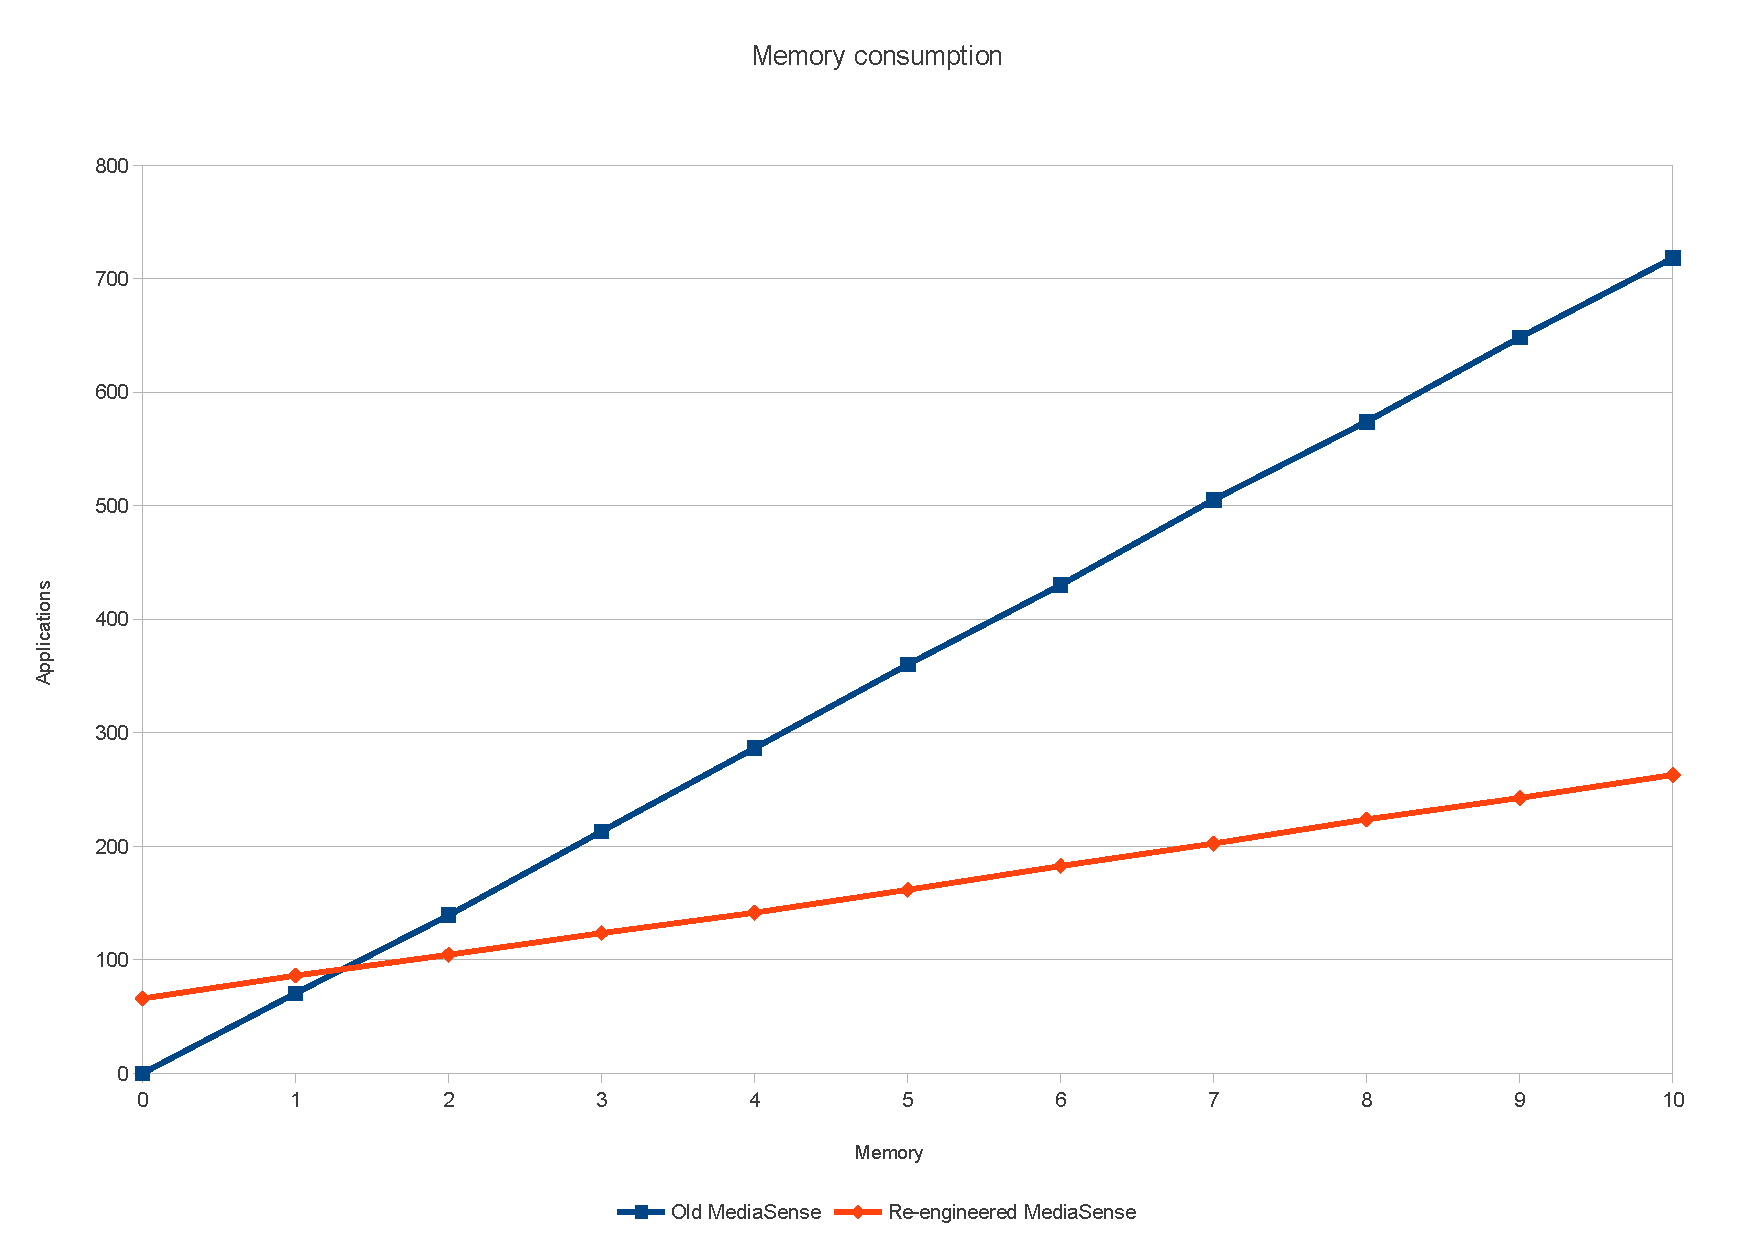
\includegraphics[scale=0.50]{part_7/test_results/memory.pdf}
\end{figure}

\begin{figure}[H]
		\centering
    	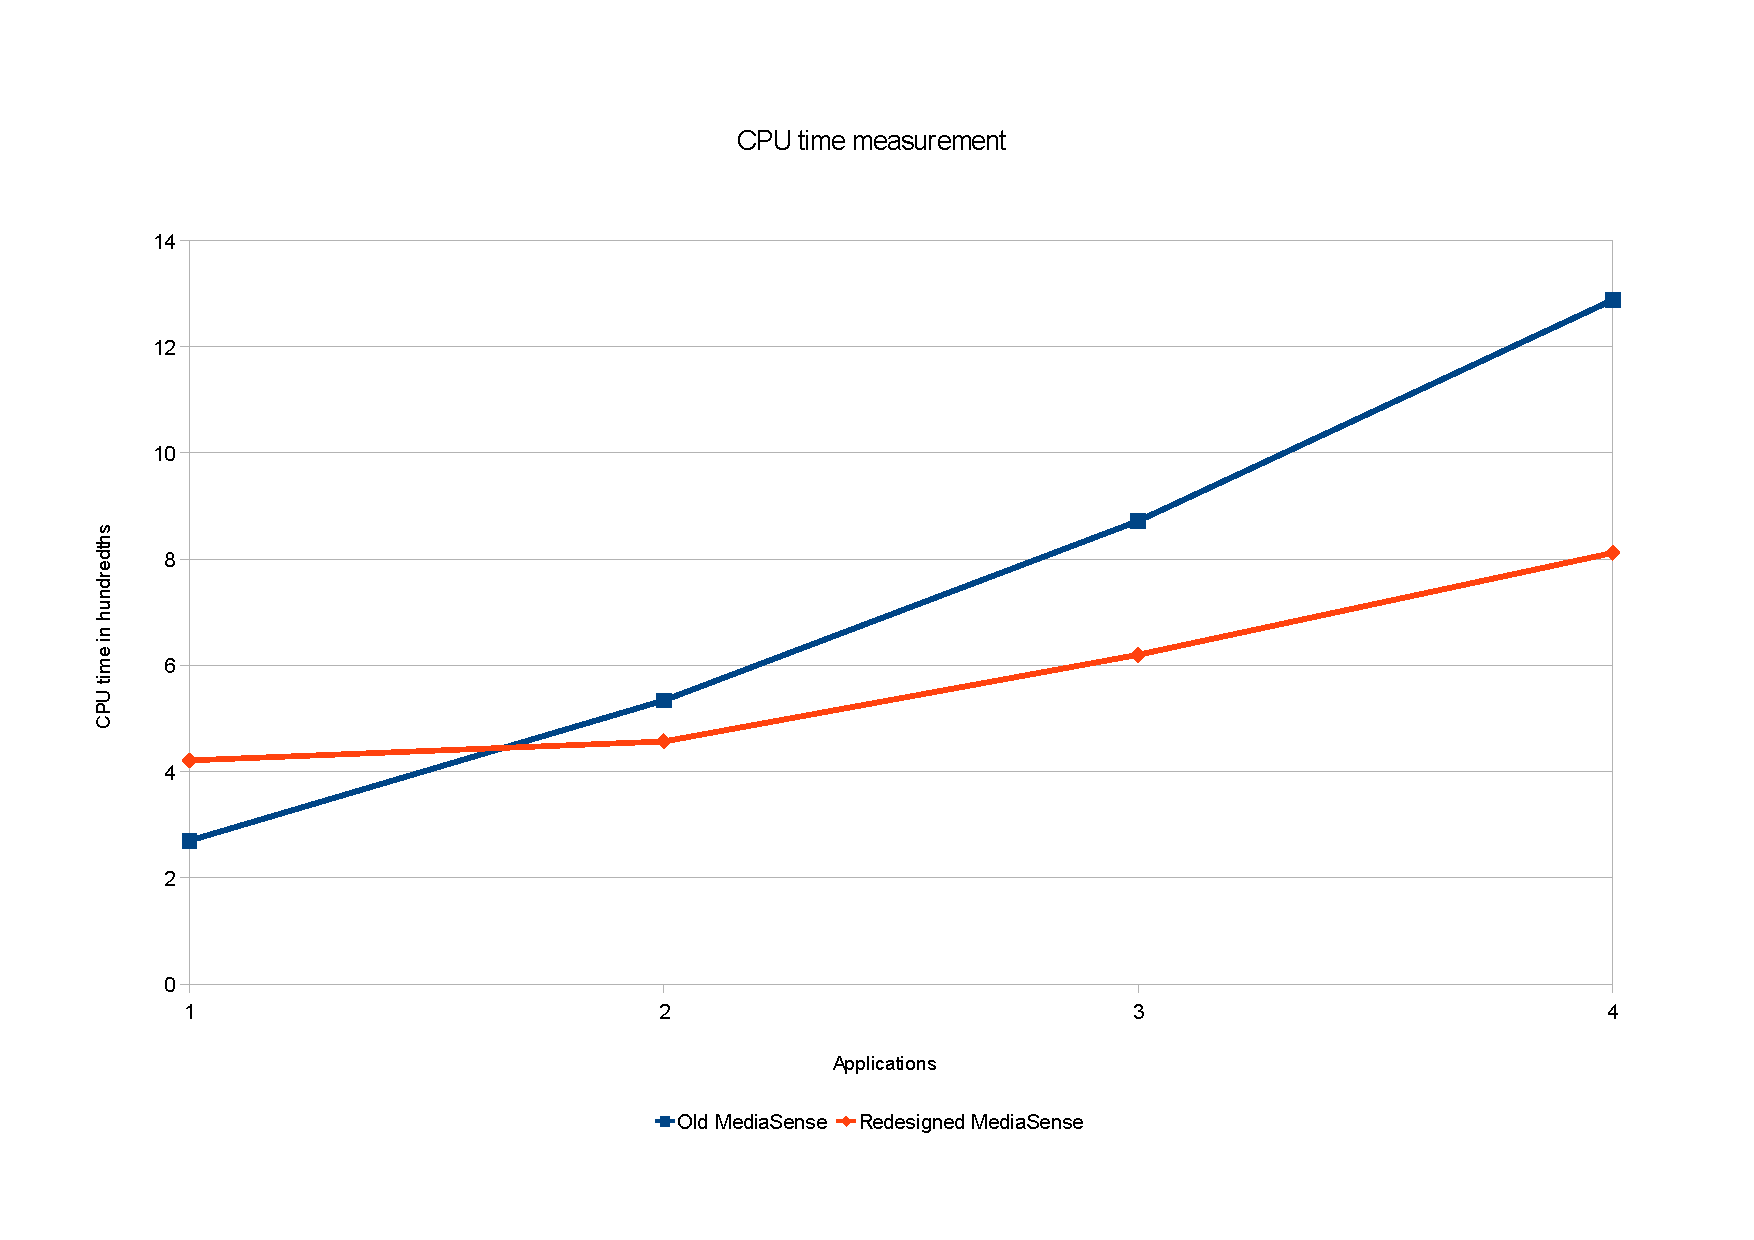
\includegraphics[scale=0.50]{part_7/test_results/cputime.pdf}
\end{figure}

\begin{figure}[H]
		\centering
    	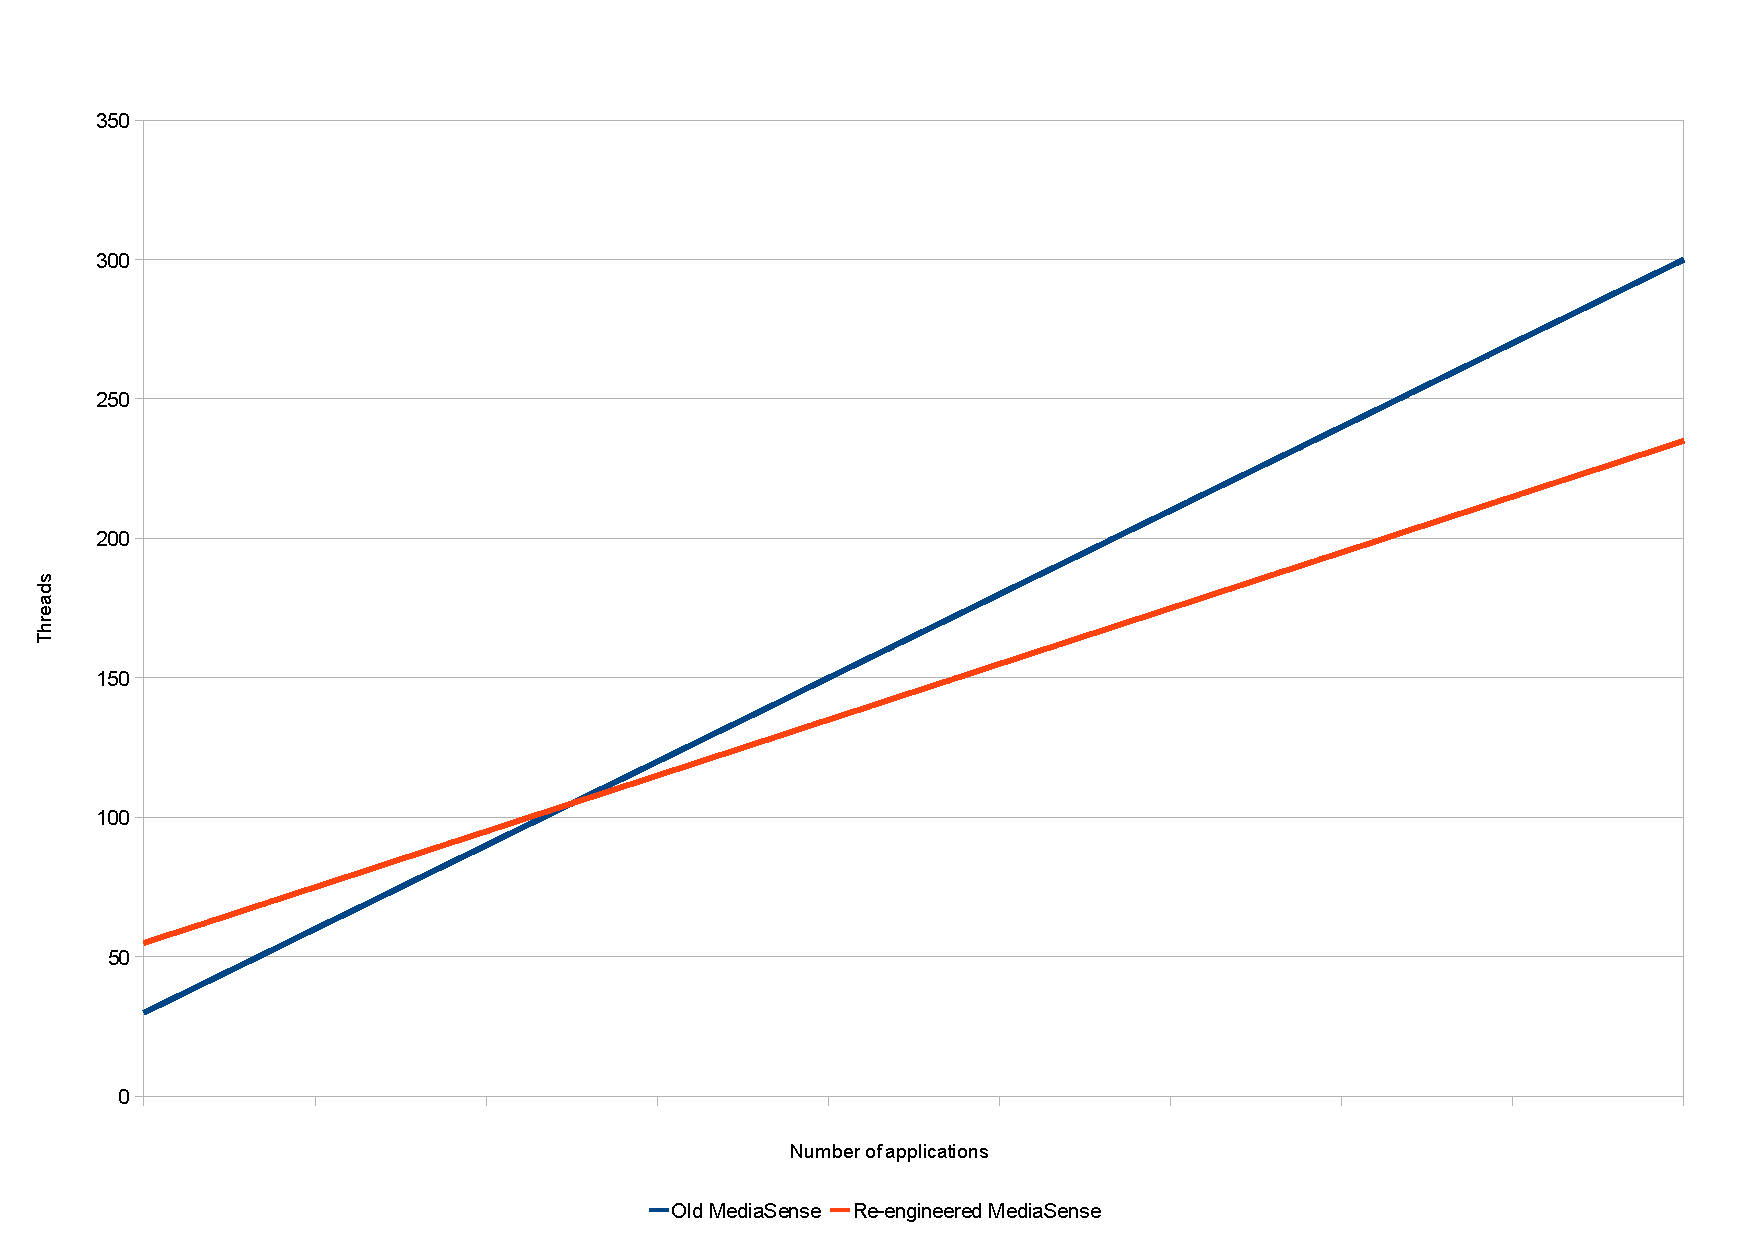
\includegraphics[scale=0.50]{part_7/test_results/threads.pdf}
\end{figure}

